%!TEX root = Problems1_main.tex

% Remove the author and date fields and the space associated with them
% from the definition of maketitle!
\makeatletter
\renewcommand{\@maketitle}{
\newpage
 \null
 \vskip 2em%
 \begin{center}%
  {\Large \@title \par}%
 \end{center}%
 \par} \makeatother

\begin{center}
\Huge University Physcis Answers 1\\[1em]
\large 23rd January 2013
\end{center}
\setcounter{section}{0}

\section{Rolling}
The first ball reaches B first.

The total displacement is the same in each case, but it is clear that the second ball will travel a greater distance. We must consider the velocity changes. For the flat sections in both cases, the velocity is the same since there is no friction so no way to loose energy. The downhill and uphill sections, however, must cause a change in velocity. 

Looking only at the second case, if we examine the average velocity, we have two sections at the initial velocity, one section of positive acceleration and one section of negative acceleration. Since, over the range of the dip, the ball must begin and end at the same velocity, these must cancel out. Thus, the total average velocity of the second path is the same as the velocity of the first.

Finally, we look at the time taken. The time to cover a distance, $s$, is
\begin{align*}
	t = \frac{s}{v}
\end{align*}
Since both paths have the same average velocity, but the second travels further, this must take longer and so the first ball reaches B first.

\section{Running}
d is the fastest route.

This is a problem of minimising the time to travel a given distance. We must take into account the fact that the runner will be able to travel faster on the tarmac than the sand, but that the longer they spend on the tarmac, the further they must travel. A compromise, then, must be made.

c (the shortest overall distance), means the runner spends too long in the sand and so is slowed down too much, however, e (the longest time on the tarmac) means the runner travels to far overall. d then is the best compromise.

This is applicable to light travelling through mediums of different density. It is the same reason that light bends when moving from air to water, or the other way round, making a straw appear to bend. The tarmac is the air in this case, where light travels faster, it then slows down at the boundary with the water, the sand.

The mathematical basis for calculating the exact route taken by the light, or runner, is called Fermat's Principle of Least Time and involves integrating the time taken given the velocity in each medium. This would be covered in first year optics.

\section{Dropping}
The bottom of the slinky will stay still. 

There are several different explanations for this effect and whole academic papers published on the subject. Simply put, it takes a finite amount of time for information to be passed from one place to another. In this case, the information is regarding the state of the top of the slinky (has it been dropped or not) and this has to be passed from the top of the slinky to the bottom before the bottom ``knows'' what state it should be in. This information travels at a maximum speed that is determined by the tension in the material of the slinky. This means that if the gravity is higher, then the tension is higher, so the information travels faster, but also the slinky falls faster.

So we have a situation where the time for the information, in the form of a pressure wave, to travel the length of the slinky, and the top of the slinky to fall the same distance, are the same. This means the end stays where it is until the information that the top has been released, and the rest of the slinky, reach that point, and then the whole slinky falls together. See a recent paper, August 2012, here http://arxiv.org/pdf/1208.4629v1

\section{Counting}
Assume the following:
\begin{itemize}
	\item The volume of an average breath is 0.5\,litres (actual value 0.3 to 2.0\,litres depending on physical activity, gender etc.)
	\item The atmosphere is roughly 10\,km high (actual value is considerably larger but majority of mass contained within 10-15\,km)
	\item The density of the atmosphere is 1.2\,$\text{kg\,m}^{-3}$ and composed entirely of nitrogen (actual value at sea level but then decreases steadily to zero, and nitrogen is 78\%)
	\item Julius Caesar lived to 50\,years (actually 55)
\end{itemize}
First we need to work out the number of molecules in the whole atmosphere, so we need the volume of the atmosphere. This is approximated as the difference between the volume of the sphere of the earth plus the atmosphere and the sphere of just the earth.
\begin{align*}
	V &= \frac{4}{3}\pi r^3 \\
	V_{atmos} &= \frac{4}{3}\pi \times (6\,300\times10^3 + 10\times10^3) - \frac{4}{3}\pi \times (6\,300\times10^3) \\
	V_{atmos} &= 5\times10^{18}\,\text{m}^3
\end{align*}
This means the mass of the atmosphere is easy to calculate,
\begin{align*}
	M_{atmos} &= \text{density} \times \text{volume} \\
	M_{atmos} &= 1.2 \times 5\times10^{18} \\
	&= 6\times10^{18}\,\text{kg} 
\end{align*}
The average atomic mass of nitrogen is 14, so
\begin{align*}
	14\,\text{g} &= 1\,\text{mol} \\
	14\times10^{-3}\,kg &= N_A\, \text{molecules} \\
	\Rightarrow 1\,\text{kg} &= \frac{N_A}{14\times10^{-3}}\, \text{molecules} \\
	&= 4\times10^{25}\, \text{molecules per kilogram} \\
	\Rightarrow N_{atmos} &= (4\times10^{25}) \times (6\times10^{18}) = 2.5\times10^{44}\, \text{molecules}
\end{align*}
For the number of molecules in each breath, we know that 1\,litre is $10^{-3}$\,m$^3$, so the number of molecules in each breath is $N_{breath}$. 
\begin{align*}
	M_{breath} &= 0.5\times 10^{-3}\times 1.2 = 6\times 10^{-4}\,\text{kg} \\
	\intertext{We know the number of molecules of nitrogen per kilogram, so}
	N_{breath} &= 4\times10^{25}\, \text{molecules per kilogram} \times 6\times 10^{-4}\,\text{kg}\\
	&= 2.4\times10^{22} \,\text{molecules}
\end{align*}
Assuming that, in the intervening time, the molecules from Caesar's last breath are now evenly distributed throughout the atmosphere, when randomly selecting a molecule from the air, there is a small chance that is was one of Caesar's last, given by
\begin{align*}
	P &= \frac{2.4\times10^{22}}{2.5\times10^{44}}
\end{align*}
But since there are such a large number of molecules in each of your breaths, this probability becomes quite high. So for each lungful of air, there is, on average,
\begin{align*}
	M &= \frac{2.4\times10^{22}}{2.5\times10^{44}} \times 2.4\times10^{22} \\
	&\approx 2
\end{align*}
molecules from Caesar's final breath.

\section{Floating}
A. No change.

An object in a fluid displaces a mass of that fluid equal to the mass of the object. Put another way, any object, wholly or partially immersed in a fluid, is buoyed up by a force equal to the weight of the fluid displaced by the object.

This means that the ice displaces a volume of water of mass equal to its own mass. As it melts, the mass of the ice (which is now part water) does not change and so it still displaces a volume of water equal in mass to the ice/water. When it has completely melted, the mass of the water that used to be ice is the same as the mass of the original ice and so displaces the same amount of water and so the level of the water does not change since the conditions are the same before and after.

B. No change. 

Adding water to the ice simply puts the ice in a state of partial melting. This case is the same as the previous case at a later moment in time when some of the water has melted. The ice and contained water still displace a volume of water equal in mass to the mass of the ice and contained water.

C. No change.

Air weighs less than water, so the ice displaces less water in the vessel, but it also does not contribute to the total amount of water in the vessel after the ice has melted.

D. Level goes down.

The nail weighs more than water, so it is displacing more water because of it. When the ice melts, the nail is released from the ice and sinks to rest on the bottom of the vessel. This means that it is now no longer displacing a volume of water equal in mass to its own mass, since it is supported by the bottom of the vessel. It now displaces only a volume of water equal to its own volume. Since it is more dense than water, this is less than before and so the water level decreases.

\section{Observing}
The observed image is found by tracing backwards, the incoming light ray. As the number of reflections made by the ray increases, the number of images increases.
\begin{figure}[ht]
  \centering
  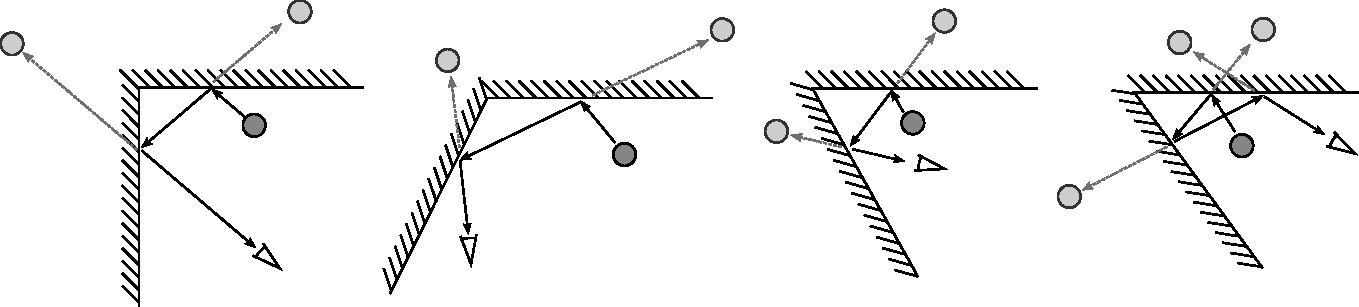
\includegraphics[width=1.0\textwidth]{mirrors_answer.pdf}
\end{figure}
When at right angles, the mirrors have the property that they reflect light rays back parallel to their angle of incidence. These mirrors are called corner- or retro-reflectors. They are used when light is required to be reflected back at the source no matter what angle they are illuminated from. They are used in bike reflectors, cats eyes (both on the road and in nature), and on the moon for use in laser based distance measurement.
